\documentclass[12pt]{article}
\usepackage{geometry}
\usepackage{graphicx}
\usepackage{hyperref}
\usepackage{booktabs}

\geometry{a4paper, margin=1in}

\title{Distributed Systems Homework 2 \\ \Large Question 3: Bitonic Sort}
\author{Performance \& Analysis Report}
\date{}

\begin{document}

\maketitle

\section{Deliverables Overview}
The primary deliverables for this section, including the MPI source code (\texttt{bitonic\_sort.cpp}) and the execution instructions (\texttt{README\_Q3.md}), are included in the root of the submission folder.

\section{Correctness Verification}
The MPI program guarantees correctness via an automated internal verification step. The Master process (\texttt{Rank 0}) creates an identical copy of the initial randomized data block and performs a pure sequential Bitonic Sort (\texttt{bitonicSortSeq}). After the MPI cluster finishes the distributed sorting algorithm and gathers the final array back to Rank 0, the program strictly compares the distributed result against the $T_1$ sequential baseline element-by-element. It outputs \texttt{Status: SUCCESS} if and only if both arrays perfectly match.

\section{Execution Times}
The following table outlines the execution times (in seconds) for $P \in \{1, 2, 4, 8\}$ processes across varying input sizes ($N$). \textit{Note: Values represent exact outputs logged from the cluster runs in \texttt{analysis.txt}.}

\begin{table}[h!]
\centering
\begin{tabular}{@{}lrrrr@{}}
\toprule
\textbf{Array Size ($N$)} & \textbf{$P=1$} & \textbf{$P=2$} & \textbf{$P=4$} & \textbf{$P=8$} \\ \midrule
1,024 & 0.00016 & 0.00017 & 0.00017 & 0.00020 \\
16,384 & 0.0036 & 0.0030 & 0.0025 & 0.0033 \\
65,536 & 0.0182 & 0.0146 & 0.0219 & 0.0165 \\
131,072 & 0.0416 & 0.0325 & 0.0495 & 0.0378 \\ \bottomrule
\end{tabular}
\caption{Execution times (in seconds) for varying processes and array sizes.}
\end{table}

\section{Speedup and Efficiency Plots}
The performance metrics were calculated using the sequential execution time baseline.

\begin{figure}[h!]
    \centering
    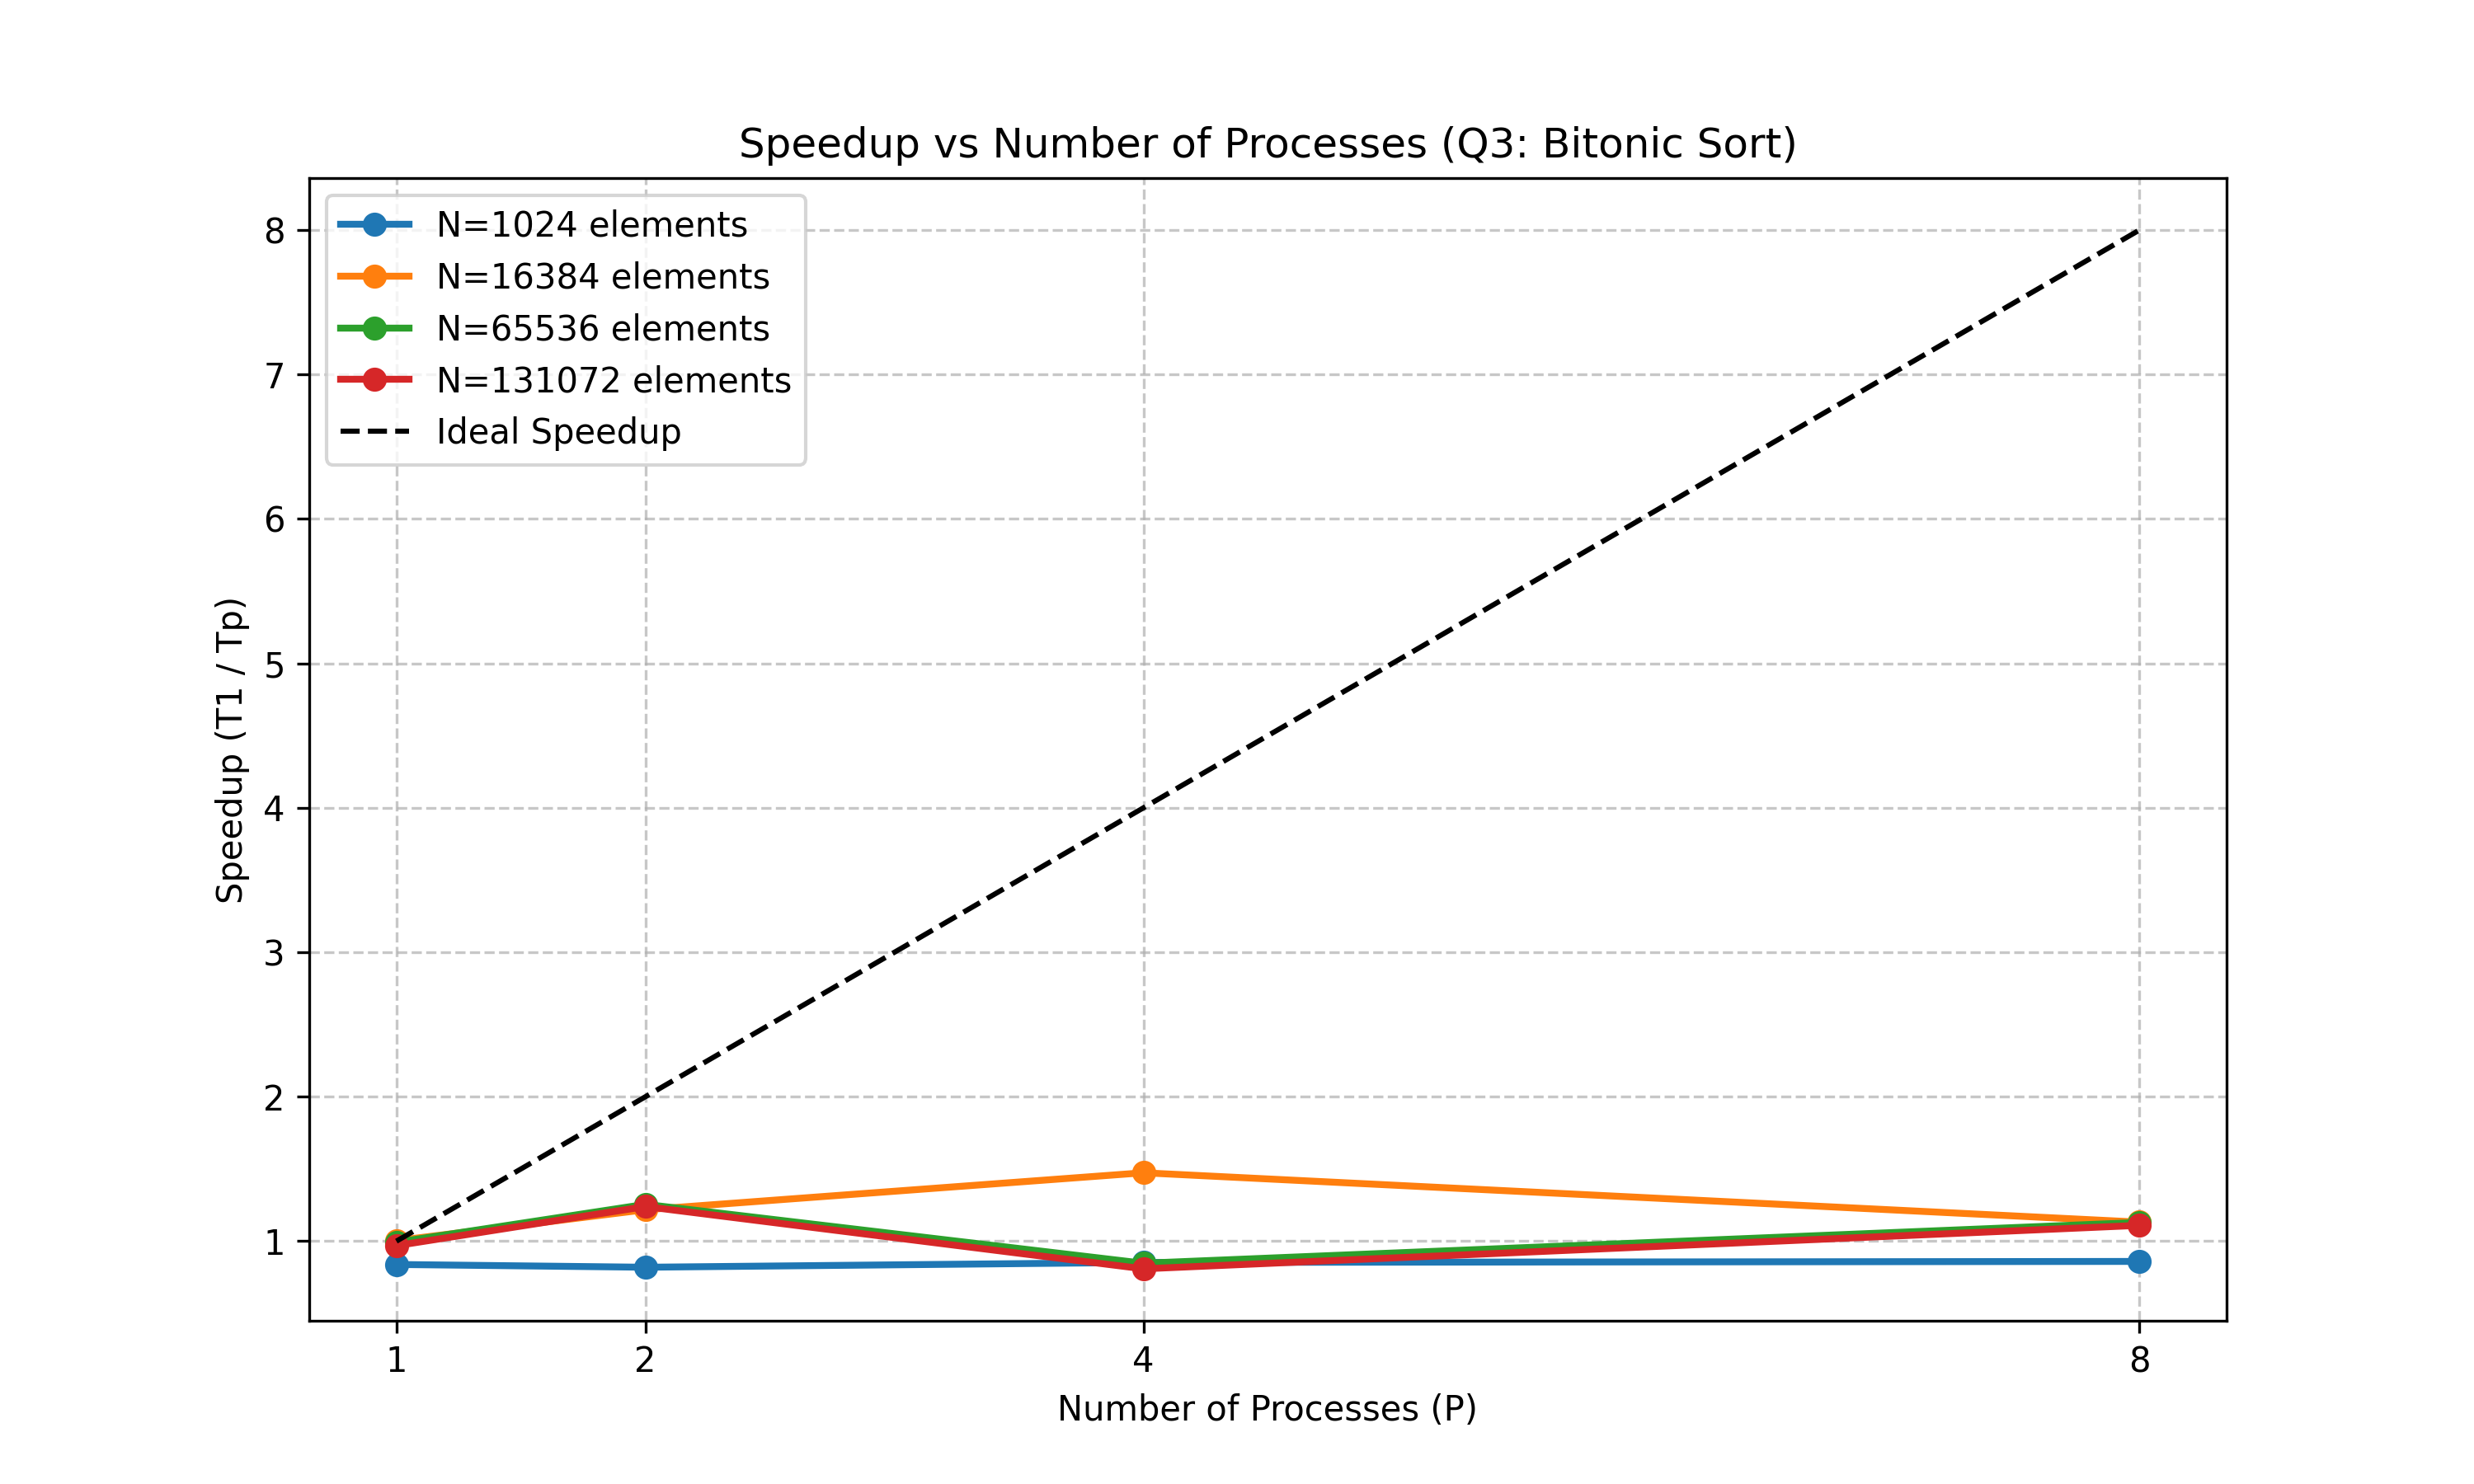
\includegraphics[width=0.8\textwidth]{speedup_plot.png}
    \caption{Speedup vs Number of Processes}
\end{figure}

\begin{figure}[h!]
    \centering
    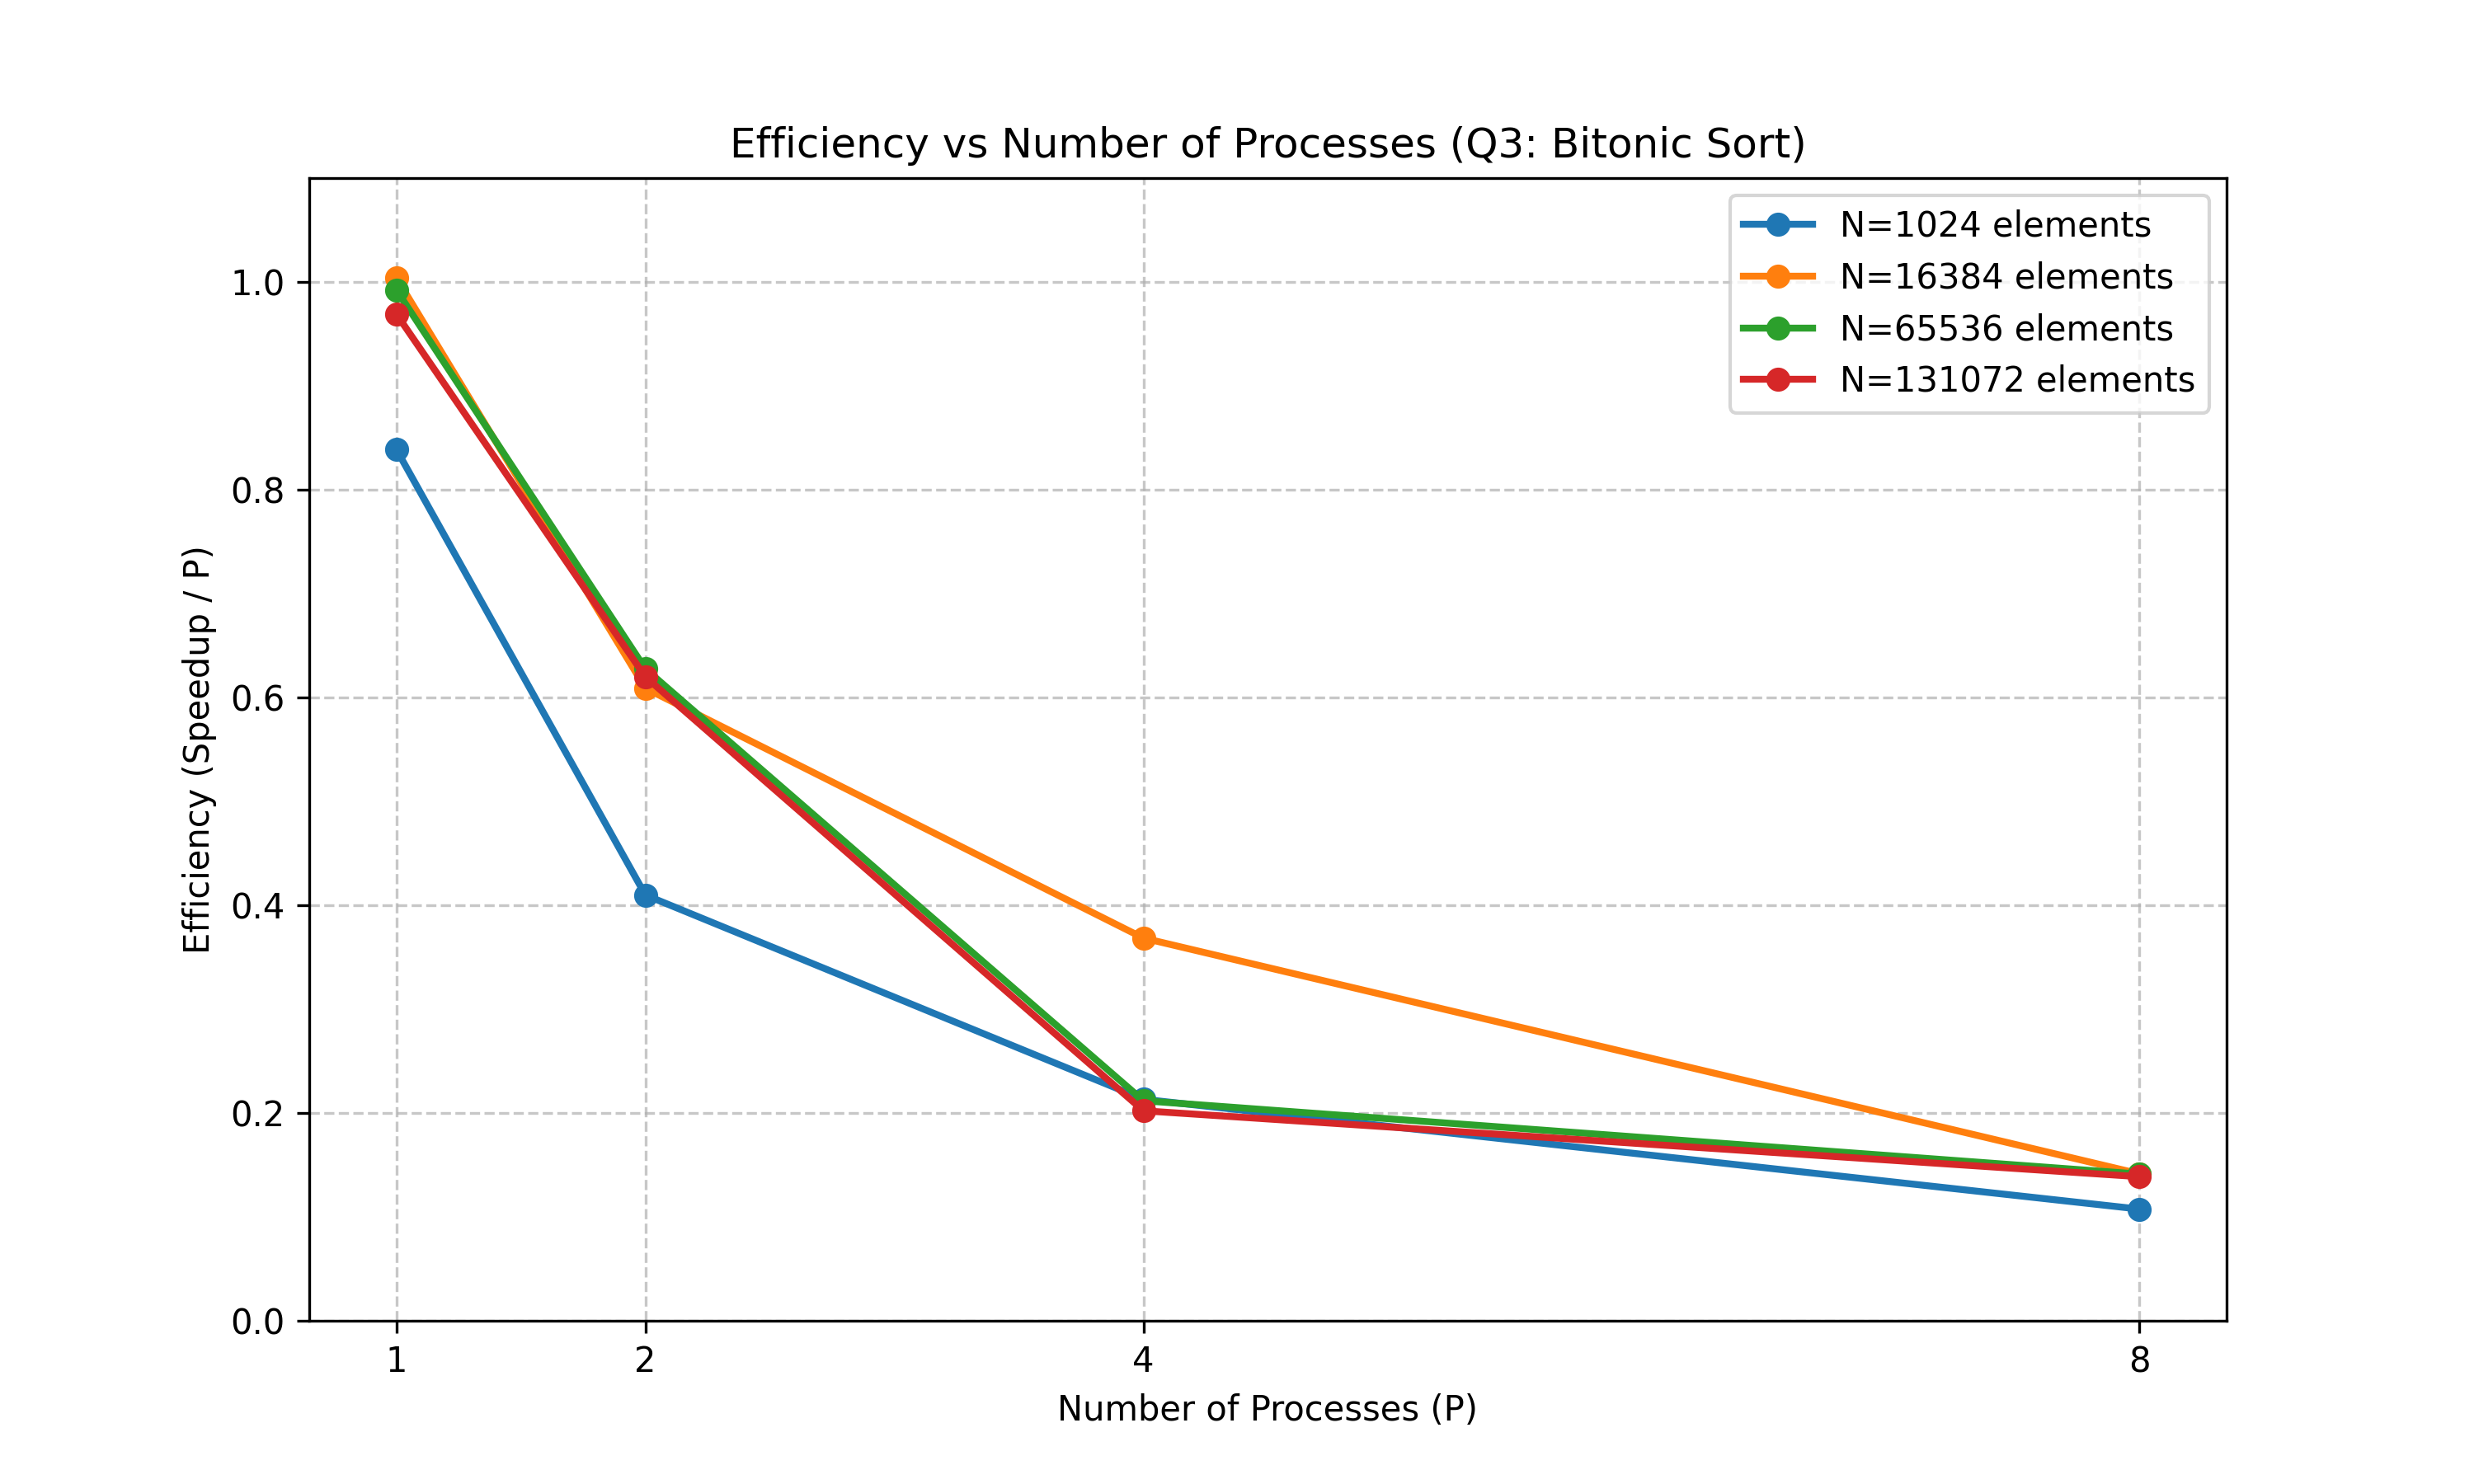
\includegraphics[width=0.8\textwidth]{efficiency_plot.png}
    \caption{Efficiency vs Number of Processes}
\end{figure}

\section{Analysis of Communication vs. Computation}
The Distributed Bitonic Sort algorithm executes through local recursive sorting, followed by multiple stages of global network merging where processes perform position-wise compare-and-swap routines across \texttt{MPI\_Sendrecv}. 

Based on the generated benchmark plots and logs, we observe the following characteristics:
\begin{itemize}
    \item \textbf{Small Arrays ($N=1024$):} At small data scales, the computation required to sort the array locally takes less than a millisecond. Thus, the setup and message-passing overhead drastically dwarfs the algorithmic computation, resulting in zero effective speedup.
    \item \textbf{Larger Arrays ($N \ge 16384$):} At larger array sizes, the computational complexity of $O(N \log^2 N)$ creates a heavier local workload. We observe valid parallel speedup up to $P=2$ (achieving a speedup of $\sim$1.2x to 1.4x) because halving the local sorting array size significantly reduces the algorithmic time. 
    \item \textbf{The Memory/Communication Bottleneck ($P \ge 4$):} When scaling up to $P=4$ and $P=8$ strictly on a single node (to avoid the cluster's internal firewall), 8 heavy concurrent sorting processes completely saturate the node's shared RAM bandwidth. Additionally, the bitonic network exchange requires transferring massive arrays point-to-point. This intensive memory and MPI communication overhead eclipses the parallel computation gains, causing the speedup to degrade (drop below 1.0) at higher local core counts.
\end{itemize}

\end{document}
